\documentclass[10pt]{article}
\usepackage{graphicx, verbatim}
\usepackage{amsmath}
\usepackage{amssymb}
\usepackage{amscd}
\usepackage{lipsum}
\usepackage{todonotes}
\usepackage[tableposition=top]{caption}
\usepackage{ifthen}
\usepackage[utf8]{inputenc}
\usepackage{graphicx}
\usepackage{caption}
\setlength{\textwidth}{6.5in} 
\setlength{\textheight}{9in}
\setlength{\oddsidemargin}{0in} 
\setlength{\evensidemargin}{0in}
\setlength{\topmargin}{-1.5cm}
\setlength{\parindent}{0cm}
\usepackage{setspace}
\usepackage{float}
\usepackage{amssymb}
\usepackage[utf8]{inputenc}
\usepackage{fancyhdr}
\usepackage{tabularx}

\usepackage{hyperref}
\hypersetup{
  colorlinks   = true, %Colours links instead of ugly boxes
  urlcolor     = blue, %Colour for external hyperlinks
  linkcolor    = blue, %Colour of internal links
  citecolor   = red %Colour of citations
}

%\fancyhf{}
\rfoot{Your Name \thepage}
\singlespacing
\usepackage[affil-it]{authblk} 
\usepackage{etoolbox}
\usepackage{lmodern}


% Notice the following package, it will help you cite papers
\usepackage[backend=bibtex ,sorting=none]{biblatex}
\bibliography{references}

\begin{filecontents*}{references.bib}

\end{filecontents*}


\usepackage{Sweave}
\begin{document}
\Sconcordance{concordance:submission.tex:submission.Rnw:%
1 50 1 1 0 63 1 1 2 1 0 5 1 1 4 2 0 1 1 1 2 1 3 1 0 1 1 3 0 1 2 8 1 1 3 %
1 0 3 2 3 0 1 2 1 3 8 0 1 2 2 1 1 3 5 0 1 2 1 6 15 1 1 3 7 0 1 3 7 0 1 %
2 1 1 1 2 4 0 1 2 2 1 1 3 2 0 1 4 2 0 1 4 5 0 1 2 3 1 1 4 6 0 1 2 5 1 1 %
2 1 0 1 2 1 0 3 1 3 0 1 2 10 1 1 2 1 0 1 3 2 0 2 1 1 3 4 0 1 2 2 1 1 13 %
15 0 1 2 1 1 1 4 3 0 1 2 5 1 3 0 1 2 9 1 1 2 1 0 2 1 3 0 1 2 1 1 1 2 5 %
0 1 3 1 2 4 0 1 2 1 3 2 0 1 2 1 0 1 2 1 0 1 1 3 0 1 2 1 1 1 3 2 0 1 2 4 %
0 1 2 1 4 3 0 1 7 6 0 1 2 1 3 5 0 1 2 1 3 2 0 1 2 8 0 1 2 7 0 1 2 11 1 %
1 2 1 0 9 1 1 2 3 0 1 2 1 4 3 0 1 2 1 0 1 3 7 0 2 2 6 0 1 1 6 0 1 2 12 %
1 1 31 32 0 1 2 7 1 1 16 18 0 1 2 1 1 1 3 2 0 2 1 1 5 6 0 1 2 2 1 1 3 6 %
0 1 2 7 1 1 2 5 0 1 2 6 1 1 8 7 0 3 1 3 0 1 2 5 1 1 2 5 0 1 2 9 1 1 3 6 %
0 1 2 9 1 1 3 6 0 1 2 8 1 1 3 2 0 1 1 1 3 7 0 2 2 5 0 2 3 2 0 2 1 3 0 1 %
2 20 1}



\title{\LARGE Coursework  \\ Module Name (CMM536)}

\author{Alexander Hall, \textit{\href{1608941@rgu.ac.uk}{1608941@rgu.ac.uk}}}
\maketitle
% \begin{flushleft} \today \end{flushleft} 
\noindent\rule{16cm}{0.4pt}
%\underline{\hspace{3cm}
\ \\
%\thispagestyle{empty}

\section{Research}

The paper that was chosen for this work is \textit{Effective and Real-time In-App Activity Analysis in Encrypted Internet Traffic Streams} \cite{Liu:2017:ERI:3097983.3098049}. The authors attempted to improve methods for classifying encrypted messaging traffic through streaming methods. Below is a review of this paper that includes problem statement, related work and methods applied.\\


\subsection{Problem Statement}

The methods presented in the reviewed paper attempt to address the growing issue of traffic analysis for messaging apps on mobile devices. Mobile and internet providers require the capability to classify traffic in order to tailor services to users and to manage load on the network. However, the rise of end to end encryption makes classification of traffic an increasingly difficult problem. It is possible to first segment and then classify encrypted traffic, however past attempts were relativley slow due to a lengthy feature extraction process. They were also intensive with respect to storage and memory due to the need to store raw packet data. The variable length of packets also affected classification accuracy. By running the clustering and classification of actual data in a streaming manner and iterativley select features from offline training data, this study sought to both decrease runtime and increase accuracy.

\subsection{Relevant Work}
The paper acknowleges previous studies \cite{Haffner:2005:AAC:1080173.1080183} \cite{4669733}  \cite{1550864} which were able to classify messaging data through the port number, protocol signature and protocol type. However, these methods are not applicable for encrypted data. Later studies \cite{5693957}, including one by the same team \cite{7377112}, were able to classify encrypted data using machine learning by segmenting traffic and then classifying it. These attempts suffered from low relative accuracy and speed. 



\subsection{Methodology}
Thw raw data used consisted of raw packets of traffic data from facebook, Whatsapp and Wechat, with the objective being to classify the usage activity (audio, location, text etc) of the data at a given point in time. The model used incorporated both offline and online (streaming) elements, with training performed offline and clustering/classification of real-world data performed in a streaming manner. The offline segment involved training up a random forest classifier with usage activity as the dependant variable. Pre-collected and labelled messaging traffic was used to train the random forest after feature extraction which involved extracting features. The data was then split into time windows and a feature selection stage used to determine the best features for clasification. The individual time windows, across the selected features, were then used to train the random forest classifier. The optimal features were also stored for use in the online stage.

The streaming stage involved streaming raw packets and extracting the optimal features (as defined offline). The data was then split into time windows which were segmented in a streaming manner using a custom implementation of KMeans clustering, referred to as recursive Constrained KMeans Clustering (rCKC). This recursivley splits clusters based on the derived property \textit{Maximal Inner Activity Similarity (IAS)}. Clusters of similar traffic are expected to have low IAS values. The individual traffic segments (note, each segment represents similar traffic) are then passed into the pre-trained random forest classifier to determine the usage activity.


\subsection{Results}
To evaluate model effectiveness, the offline portion of the model was first conmpared to other baseline models; followed by a comparison of the full streaming model (pre-trained offline) against previous approaches. The Hierachical Random Forest classifier (HRF) was assessed using two accuracy metrics: Total Duration Accuracy (TDA) and Total Volume Accuracy (TVA). Both accuracy metrics are higher for the proposed HRF classifier across all three messaging services. 
The entire model, including the streaming section, was then tested against a number of baseline models. The TDA and TVA for the model were higher than any of the other baseline models.Along with higher accuracy, the new model exhibited a greatly reduced runtime compared to the baseline models, with a 14.3x speedup compared to the next most accurate model. 

\subsection{Conclusion}
The model presented was able to classify encrypted messaging traffic with a higher accuracy than any of the previously tested models. By streaming the testing stage, and pre-seleting the most important features, classification speed was greatly increased. This increases the viability of the model for real-world applications where real-time analysis of large volumes of messaging data is a requirement.
For the offline classifier, it should be noted that the result does not appear to be statistically significant from the basline models given the figures provides as the confidence intervals are seen to overlap. The authors do not state the confidence level used so it is not possible to infer the true significance of the result. Likewise,  it is stated that the result for the stream classifier was 'significantly' higher but it is unclear whether the authors are inferring statistical significance as there is no mention of repeatability and no confidence intervals are shown on the overall results plot.

\pagebreak


\section {Data Streams}

The dataset analysed here is the Dota 2 game results dataset, available at\\
\url{ https://archive.ics.uci.edu/ml/datasets/Dota2+Games+Results}

The data is taken from the popular online multiplayer game Dota 2. This game is played between two teams of five players each. Each individual player plays as a 'hero' (selected by the player themselves). The two teams then compete to defend their respective bases. The first team to destroy the others base wins.\\

The dataset was chosen because Dota 2 is widely seen as a challenging problem in the field of AI \cite{7828640}. Following the success of Alphago at the boardgame go in 2016 \cite{8295075}, Dota 2 is seen by many as the next challenge as no AI has yet been able to beat a leading human team. As with any well designed computer game, balancing is key. In this case, it is a requirement that any given team of heroes should perform equally well as any other team (given players of equal skill). With over 100 different heroes available, each with their own strengths and weaknesses, balancing is a challenging problem for the game design team. If any given set of heros can be shown to have an advantage over another set, this could be used by human, or AI, players to gain an advantage over the other team. This analysis, therefore doesn't seek to predict whether a team will win with a high degree of accuracy (if that were possible, Dota 2 would be a poorly balanced and unsuccessful game); rather we seek to find any marginal advantage beter than random guessing.\\


With 116 dimensions, the dataset is large enough to demonstrate the potential benefits of streaming, but small enough to classify in a non-streaming manner on a single machine. 

\subsection{Data Exploration}

The dataset itself contains data from 102944 individual games. The dependant variable is a factor with levels 1 and -1, with 1 representing a win for the first team and -1 representing a win for the second team. 114 columns each represent an individual hero. If that hero was present in the first team, the respective heros column has a value of '1'; or '-1' if it was present in the second team. A '0' in a heros column means that hero was not present in either of the teams for that game.
Other independant variables are present in the form of game type, game mode and geographic data; but these were excluded for the final analysis as this study focuses solely on game balancing through choice of hero.\\

To study the dataset in more detail, let's load it into the workspace, along with the required libraries. The original dataset, as downloaded, is already split into a training and testing set. However, in order to ensure the split as indeed random and stratified, the data was re-combined into a single dataset.

\begin{Schunk}
\begin{Sinput}
> library(dplyr)
> library(rjson)
> library(caret)
> library(randomForest)
> library(ROCR)
> library(dummies)
> #read in the train and test datasets and combine 
> 
> df1 <- read.csv('dota_dataset\\dota2Train.csv')
> df2 <- read.csv('dota_dataset\\dota2Test.csv')
> names(df2) <- names(df1)
> #combine the original datasets to a single dataframe
> df <- rbind(df1,df2)
> rm(df1,df2)
\end{Sinput}
\end{Schunk}

Looking at the basic structure of the data we note the following (outputs not shown in pdf due to size):
 
\begin{itemize}
  \item The typing is incorrect as imported - the types should all be factors
  \item The dataset is quite sparse
  \item The columns are not named. They are defined in the readme for the dataset so we will add names later
\end{itemize}

\begin{Schunk}
\begin{Sinput}
> library(xtable)
> print(xtable(head(df)))
> str(df)
> names(df)
\end{Sinput}
\end{Schunk}
Let's also check the size of the dataset:
\begin{Schunk}
\begin{Sinput}
> #record number of rows and columns
> paste('number of columns =' , ncol(df) , '. number of rows =', nrow(df))
\end{Sinput}
\begin{Soutput}
[1] "number of columns = 117 . number of rows = 102942"
\end{Soutput}
\end{Schunk}

Now let's check the class distribution (ie do we have an approximately equal number of team 1 wins as team 2 wins?).
The distribution is indeed close to equal so we do not need to worry about class imbalance later on. It is interesting to note there is some imbalance, the reason for this is not clear but probably has something to do with the manner in which the data was collected.
\begin{Schunk}
\begin{Sinput}
> #check value distribution of response variable column
> table(df[,1])
\end{Sinput}
\end{Schunk}

% latex table generated in R 3.4.3 by xtable 1.8-2 package
% Sun Apr 22 18:14:40 2018
\begin{table}[ht]
\centering
\begin{tabular}{rr}
  \hline
 & V1 \\ 
  \hline
-1 & 48658 \\ 
  1 & 54284 \\ 
   \hline
\end{tabular}
\end{table}

An advantage of this dataset is there are no missing values. This is not surprising as the data was captured using the Dota 2 API. Here we also check that each team has an equal number of heroes which is a requirement for a game:

\begin{Schunk}
\begin{Sinput}
> #check for missing values (there are none)
> sum(complete.cases(df))==nrow(df)
\end{Sinput}
\begin{Soutput}
[1] TRUE
\end{Soutput}
\begin{Sinput}
> #check there are equal number of heroes present in each team (hero values for all rows should sum to zero)
> sum((rowSums(df[5:ncol(df)]))) == 0
\end{Sinput}
\begin{Soutput}
[1] TRUE
\end{Soutput}
\end{Schunk}

As discussed above, some preprocessing is required. First, we convert all numeric columns to factors:
\begin{Schunk}
\begin{Sinput}
> df[sapply(df, is.numeric)] <- lapply(df[sapply(df, is.numeric)], as.factor)
\end{Sinput}
\end{Schunk}

The column names are added in two stages. The first four columns are named manually as specified in the dataset description.\\
The remaining columns represent the individual heros. The column names are extracted from the .json file supplied with the dataset:
\begin{Schunk}
\begin{Sinput}
> #add column names to the first few columns
> names(df)[1:4] <- c('won','cluster_id','game_mode','game_type')
> #populate the other column names
> #load in json file and use it to populate column names
> hero_names <- fromJSON(file ="dota_dataset\\heroes.json")
> for ( i in c(1:length(hero_names$heroes))){
+   names(df)[i+4] <- hero_names$heroes[[i]]$name
+ }
\end{Sinput}
\end{Schunk}


Here we drop columns that are not related to heros (this analysis is concerned only with hero choice so we drop game type and location related columns). 
One column has the same value for every entry. This was noticed during the analysis stage. The column represents a mandatory hero which muct be included in the team. Since it conveys no information it is dropped:
\begin{Schunk}
\begin{Sinput}
> #drop unwanted columns
> df <- df%>%
+   select(-c(lina, cluster_id , game_mode , game_type))
\end{Sinput}
\end{Schunk}


To visualise the dataset a little more clearly, the number of times each hero was picked by a team can be plotted. This gives us an idea of how popular each hero is, and may explain any particularly important variables later on. It also gives us a good indication of the general 'spread' of the data and whether the 'home' and 'away' teams tend to behave similarly. We require similar behaviour between the teams to ensure there is no bias in the results:

\begin{Schunk}
\begin{Sinput}
>#check variable balancing
>numeric_df <- sapply(df,function(x){as.numeric(as.character(x))})%>%
+  as.data.frame()%>%
+  select(-seq(1,4))

>#get number of instances of each hero for home team
>home_team_heros <- ifelse(numeric_df==1,1,0)%>%
+  colSums()%>%
+  as.data.frame()

>home_team_heros$name <- row.names(home_team_heros)

>ggplot(home_team_heros,aes(x=name,y=.))+
+  geom_bar(stat="identity")+
+  theme(axis.text.x = element_text(angle = 90, hjust = 1,size=7))+
+  labs(title="number of times each hero was chosen by the home team")+
+  xlab("hero name")+
+  ylab("number of games the hero was picked")


>#get number of occurances for each away team hero
>away_team_heros <- ifelse(numeric_df==-1,1,0)%>%
+  colSums()%>%
+  as.data.frame()

> away_team_heros$name <- row.names(away_team_heros)

>ggplot(away_team_heros,aes(x=name,y=.))+
+  geom_bar(stat="identity")+
+ theme(axis.text.x = element_text(angle = 90, hjust = 1,size=7))+
+  labs(title="number of times each hero was chosen by the away team")+
+  xlab("hero name")+
+  ylab("number of games the hero was picked")
\end{Sinput}
\end{Schunk}


\begin{figure}[H]
\begin{center}
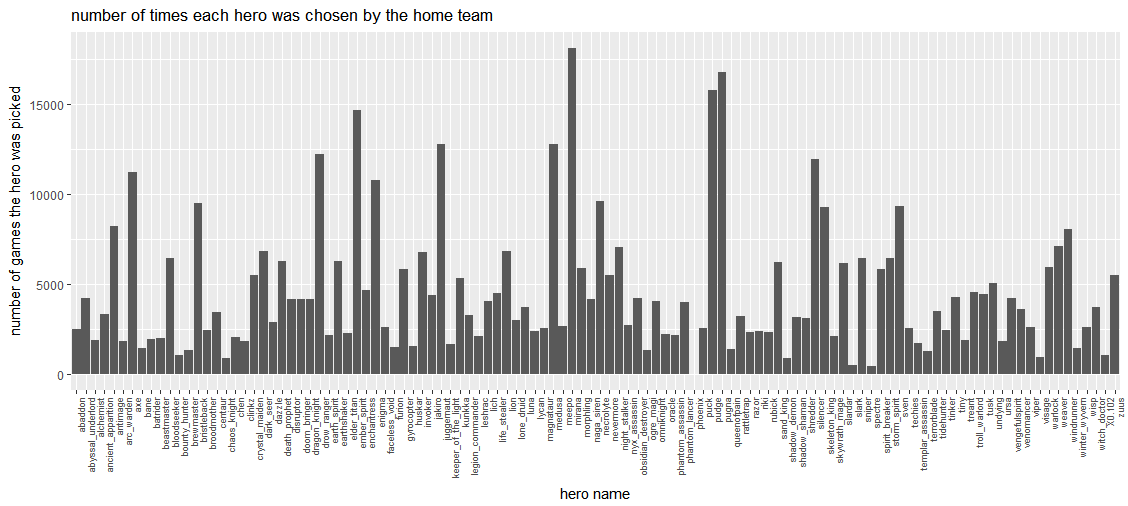
\includegraphics{home_team}
\caption {Number of matches in which the home team picked each hero}
\label{home}
\end {center}
\end {figure}

\begin{figure}[H]
\begin{center}
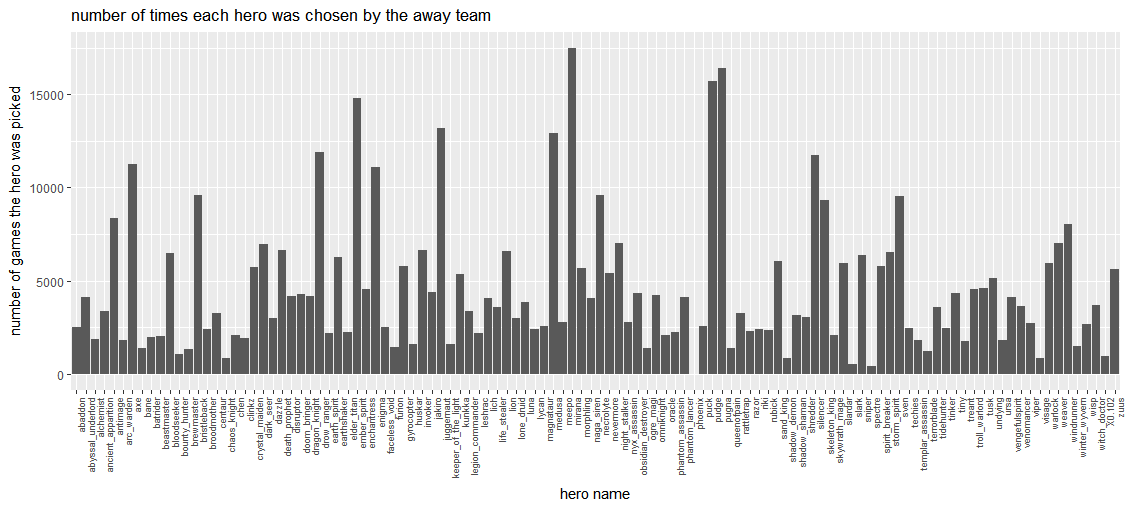
\includegraphics{away_team}
\caption {Number of matches in which the away team picked each hero}
\label{away}
\end {center}
\end {figure}

Inspecting the two plots above, there are two noteable features in the dataset:

\begin{itemize}
\item Some heros are extremely popular while others are barely used. The most popular heros will be considered when studying variable importance, since a high variable importance corresponding with a commonly used hero doesn't tell us much about underlying trends in the data.
\item The distribution of hero choice is almost identical for the home and away teams. This suggests that teams were indeed chosen randomly and there was no skill or behavioural bias. This means any trends identified in the data are likely to be due to the game design itself rather than a skill disparity between teams.
\end{itemize}

\subsection{Build Classifier}
The dataset is now split into training, testing and validation sets. 60\% of the data is used for training with 20\% used for testing and validation respectivley:
\begin{Schunk}
\begin{Sinput}
> set.seed(57)
> # Split into train test and validation sets
> index <- sample(c(1:3), size = nrow(df), replace = TRUE, prob = c(.6, .2, .2))
> df_train <- df[index == 1,]
> df_test <- df[index == 2,]
> df_valid <- df[index == 3,]
\end{Sinput}
\end{Schunk}

A random forest classifier was used to classify the data. This model was chosen for two main reasons:
\begin{itemize}
  \item With only 3 main tuneable parameters, random forests often require less tuning than other model types.
  \item For high dimensional data, a SVM would typically perform well, however with over 100000 rows in the dataset, runtime would probably be significant. Random forests typically also perform well on high dimensional data. \cite{GENUER201728}
\end{itemize}


Rather than simply training up and testing a single model, some parameter tuning was carried out. The mtry and nodesize parameters were tuned using a tuning grid. Although this gave only 9 different combinations of hyperparameters, it serves as a demonstration of how model selection is achieved.

Here, a parameter grid is defined and stored as a dataframe to be accessed as each candidate model is trained
\begin{Schunk}
\begin{Sinput}
> num_attributes <- ncol(df_train)
> #build a parameter grid
> # Random forest
> mtry <- as.integer(c(num_attributes * 0.25, num_attributes / 3, num_attributes * 0.5, num_attributes * 0.8))
> nodesize <- c( 3, 5, 20)
> ntree <- c(200)
> PG<- as.data.frame(expand.grid(mtry=mtry, nodesize=nodesize,
+                                          ntree=ntree, stringsAsFactors=F))
\end{Sinput}
\end{Schunk}
Now, we train up a random forest on the training set for each combination of parameters in the parameter grid. \\
For each combination of parameters, the resulting model is tested on the evaluation set and the accuracy calculated.
The resulting accuracy from each parameter combination is saved in the 'Accuracy' column of the parameter grid table \textit{full output not shown here for brevity}:
\begin{Schunk}
\begin{Sinput}
>set.seed(57)
> for (i in c(1:nrow(PG))){
+   mtry <- PG[i, "mtry"]
+   nodesize <- PG[i, "nodesize"]
+   ntree <- PG[i, "ntree"]
+ 
+   temp_model <- randomForest(formula(df_train) , data=df_train, mtry=mtry, ntree=ntree, nodesize=nodesize)
+   predictions <- predict(temp_model , df_valid)
+   cm<- confusionMatrix(predictions,df_valid$won)
+   accuracy <- cm$overall['Accuracy']
+   PG[i,'Accuracy'] <- accuracy
+   print(i)
+ }
\end{Sinput}

\end{Schunk}

The parameters which produced the best model are selected and that model is evaluated on the testing set to give a final accuracy for the random forest classifier.
\begin{Schunk}
\begin{Sinput}
> #assess best model on test set
> PG <- PG%>%
+   arrange(desc(Accuracy))
> mtry <- PG[1, "mtry"]
> nodesize <- PG[1, "nodesize"]
> ntree <- PG[1, "ntree"]
>set.seed(57)
> best_model <- randomForest(formula(df_train) , data=df_train, mtry=mtry, ntree=ntree, nodesize=nodesize , importance=T)
> predictions <- predict(temp_model , df_valid)
> confusionMatrix(predictions,df_valid$won)
\end{Sinput}
\begin{Soutput}
Confusion Matrix and Statistics

          Reference
Prediction   -1    1
        -1 4019 3194
        1  5548 7442
                                          
               Accuracy : 0.5673          
                 95% CI : (0.5604, 0.5741)
    No Information Rate : 0.5265          
    P-Value [Acc > NIR] : < 2.2e-16       
                                          
                  Kappa : 0.1213          
 Mcnemar's Test P-Value : < 2.2e-16       
                                          
            Sensitivity : 0.4201          
            Specificity : 0.6997          
         Pos Pred Value : 0.5572          
         Neg Pred Value : 0.5729          
             Prevalence : 0.4735          
         Detection Rate : 0.1989          
   Detection Prevalence : 0.3570          
      Balanced Accuracy : 0.5599          
                                          
       'Positive' Class : -1              
\end{Soutput}
\end{Schunk}

The final accuracy of \textbf{56.7\%} is a reasonable result since an ideal game should be completely unpredictable (ie accuracy=50\%). Of course, repeatibility is a concern - this result could simply have occurred due to chance. The next section does address this by demonstrating a classifier which continually improves as more data is added.\\

The ROC curve for the predictions is plotted below, with an \textbf{AUC of 0.579}. Again, this is far from a perfect classifier but does suggest some bias in the game which could potentially be exploited by a sufficiently well-trained AI:


\begin{figure}[H]
\begin{center}
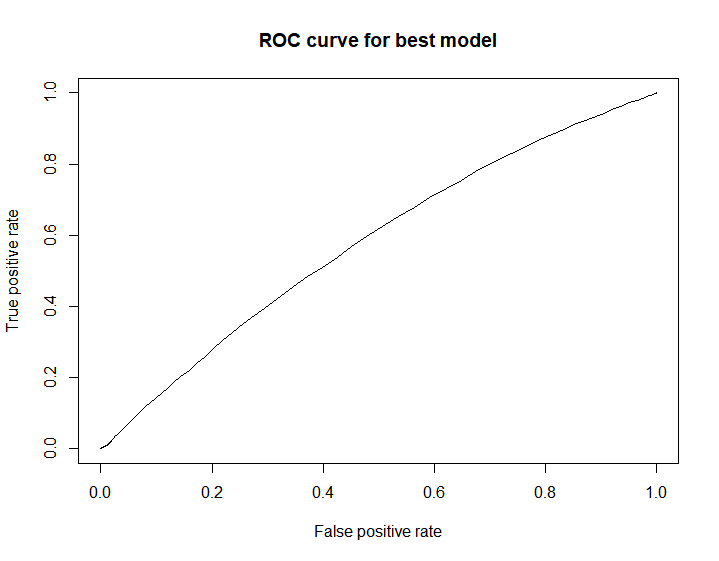
\includegraphics{roc}
\caption {ROC curve for Random Forest classifier}
\label{fig02}
\end {center}
\end {figure}


The variable importances are also of interest. In this case, each variable represents whether a particular character was used by the team, or the opposing team. So, plotting the importance of each character gives insights into any exploits that could be used to beat a team (ie by selecting or not selecting that hero). The realtive importances of the top 2 most important heroes are plotted below:

\begin{Schunk}
\begin{Sinput}
>#save variable importances
>varImps <- varImp(best_model)
>colnames(varImps) <- c('importance'," ")
>varImps <- varImps[order(-varImps$importance),] 
>varImps$names <- rownames(varImps)

>#lock in factor levels to maintain order
>varImps$names <- factor(varImps$names, levels = varImps$names)

>ggplot(varImps[1:20,],aes(x=names,y=importance))+
+  geom_bar(stat="identity")+
+  theme(axis.text.x = element_text(angle = 25, hjust = 1))+
+  labs(title="variable importance for Random Forest Model")

\end{Sinput}
\end{Schunk}

\begin{figure}[H]
\begin{center}
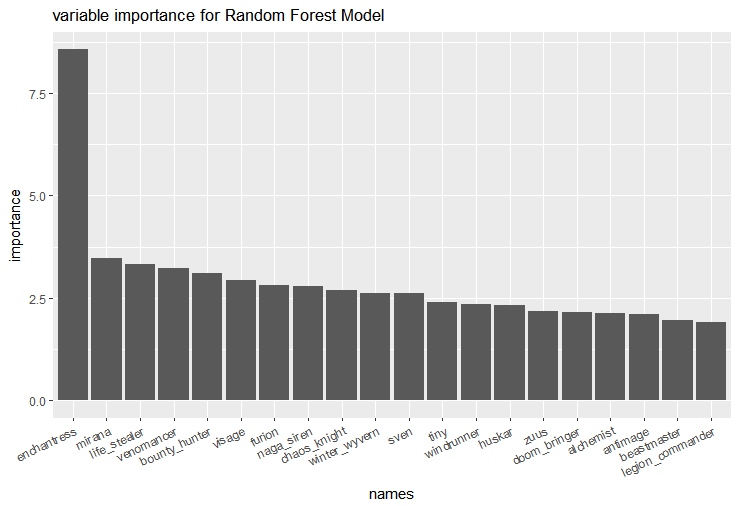
\includegraphics{vis}
\caption {variable importances of top 20 most important hero choices for Random Forest classifier}
\label{fig002}
\end {center}
\end {figure}

The variable importances give an interesting insight into how the model predicted a win/no win for the home team. Relative importance is not equal for all heroes - it declines steadily for the top 20. However, one hero in particular - 'enchantress', is dominant. Whether a team selects this hero or not has more than double the relative bearing on the final result than any other hero choice. Given additional time and resources it may be possible to learn more about any possible exploits that could be derived from this information. Presumably this hero performs disproportionately well or poorly against other specific heros and further analysis may be able to reveal why this is so.\\

It should also be noted that the 'enchantress' hero was not particularly popular or unpopular (\ref{home}), which further suggests this hero is of high importance.


  

\subsection{Build Stream Classifier}

The classifier in the previous section required over two hours of runtime for a full parameter tuning run. It may be possible to achieve a similar accuracy with just a subset of the original dataset. To ascertain whether this is the case, a streaming classifier was produced which incrementaly trains and tests a model on chunks of the dataset. This also has the advantage of preventing memory overflow since the whole dataset need not be saved in memory.

First the required libraries are loaded:
\begin{Schunk}
\begin{Sinput}
> library(data.table)
> library(RMOA)
> library(stream)
\end{Sinput}
\end{Schunk}

A validation set will not be used in this case since the aim is to demonstrate a streaming classifier; parameter tuning was demonstrated in the above section. So, the validation and testing set from the above section are combined to create a new testing set. The stream classifier will therefore be trained on 60\% of the original dataset:
\begin{Schunk}
\begin{Sinput}
> df_test <- bind_rows(df_test,df_valid)
> 
\end{Sinput}
\end{Schunk}
Several classifier types were tried but that which gave the quickest improvement in accuracy was the 'Ozaboost' classifier. This is a boosted model created specifically for streaming \cite{6934280}. A Hoeffding tree is used as the base learner.
\begin{Schunk}
\begin{Sinput}
> mymodel <- OzaBoost(baseLearner="trees.HoeffdingTree", ensemblesize=30)
\end{Sinput}
\end{Schunk}
A stream object is created to pass the data incrementally to the model. It was decided to stream data in chunks of 100 instances. For the training set of ~60000 rows, this will give ~600 chunks overall. The dataset has over 100 dimensions so 100 rows should contain enough data for the model to meaningfully update itself on every iteration.
\begin{Schunk}
\begin{Sinput}
> # Create a stream 
> dfStream <-datastream_dataframe(data=as.data.table(df_train))
> # other variables for training
> chunk <- 100
> #use the chunk size and size of the training set to define the number of turns required for training
> turns <- (nrow(dfStream$data)/chunk)-1
> turns <- floor(turns)
\end{Sinput}
\end{Schunk}
We make a similar stream object for the testing data. This will allow for testing concurrent to training ie, the model will be tested after every training iteration. This will allow for early stopping if a desired accuracy is reached before the full dataset has been used for training.\\
Note, the size of the testing chunks is defined by taking the size of the training chunks and scaling it down in proportion to the test/training set size. This ensures there are an equal number of training and testing chunks, so testing can be carried out after every training iteration.
\begin{Schunk}
\begin{Sinput}
> #make a test stream
> test_stream <- datastream_dataframe(data=as.data.table(df_test))
> # other variables for testing
> test_chunk <- floor(100 / (nrow(df_train)/nrow(df_test)))
\end{Sinput}
\end{Schunk}
Training is performed on a single chunk of data. This is achieved by retrieving a chunk from the stream object. The chunk is then used as training data for the model defined above:
\begin{Schunk}
\begin{Sinput}
> ## first sample (train) - retrieves first 100 records ##
> set.seed(57)
> sample <- dfStream$get_points(dfStream, n = chunk,
+                               outofpoints = c("stop", "warn", "ignore"))
> ## Train the first chunk
> 
> myboostedclassifier <- trainMOA(model = mymodel,
+                                 formula = won ~.,
+                                 data = datastream_dataframe(sample))
\end{Sinput}
\end{Schunk}
A single chunk of test data is also taken to be used for testing on this initial training iteration:
\begin{Schunk}
\begin{Sinput}
> test_sample <- test_stream$get_points(test_stream, n = test_chunk,
+                                       outofpoints = c("stop", "warn", "ignore"))
\end{Sinput}
\end{Schunk}
The test sample is used to evaluate the accuracy of the initial training run. It is as good as random guessing, so unsurprisingly more data will be required to build a useful classifier:
\begin{Schunk}
\begin{Sinput}
> ## Do some prediction to test the model
> predictions <- predict(myboostedclassifier, test_sample)
> table(sprintf("Actuals: %s", test_sample$won),
+       sprintf("Predicted: %s", predictions))
\end{Sinput}
\begin{Soutput}
              Predicted: -1 Predicted: 1
  Actuals: -1            17           13
  Actuals: 1             20           15
\end{Soutput}
\begin{Sinput}
> # calculate accuracy
> cat("Accuracy is: ", sum(predictions==test_sample$won)/nrow(test_sample)*100,"%")
\end{Sinput}
\begin{Soutput}
Accuracy is:  49.23077 %
\end{Soutput}
\end{Schunk}
The results for each training/testing iteration will be held in a vector for later analysis:
\begin{Schunk}
\begin{Sinput}
> # hold results in a vector
> accuracies <- c()
> #reset the test stream 
> test_stream$reset()
\end{Sinput}
\end{Schunk}
Now the model is incrementally trained and tested by feeding in chunks sequentially. For each iteration a training chunk is presented and the model is incrementally trained on that chunk. Then a testing chunk is presented to assess the performance of the model for each iteration, printing the current accuracy to the console. \textit{Full output not included in this document for brevity}.

\begin{Schunk}
\begin{Sinput}
>#train over the stream
>set.seed(57)
>for (i in 1:turns){
>  # next sample
> sample <- dfStream$get_points(dfStream, n = chunk,
+                               outofpoints = c("stop", "warn", "ignore"))
>  test_sample <- test_stream$get_points(test_stream, n = test_chunk,
+                                       outofpoints = c("stop", "warn", "ignore"))
>  ## Update the trained model with the new chunks
>  myboostedclassifier <- trainMOA(model = myboostedclassifier$model,
+                                  formula = won ~ .,
+                                  data = datastream_dataframe(sample),
+                                  reset = FALSE,trace = FALSE)
>  cat("chunk: ",i,"\n")
  
>  predictions <- predict(myboostedclassifier, test_sample)
>  # calculate accuracy
>  accuracies[i] <- sum(predictions==test_sample$won)/nrow(test_sample)*100
>  if(i %% 100 = 0){
>  cat("chunk ",i," accuracy = ",accuracies[i],"%","\n")
>  }
>}

\end{Sinput}
\end{Schunk}

The final accuracy achieved was 58.1\%, which is actually higher than for the best non-streaming model. This may be due to the use of a different model type which performed better on the given dataset. This is also a reasonably high accuracy for this problem - as stated earlier, anything above 50\% is considered a positive result since an ideal game should be perfectly balanced.

The improvement in accuracy with training/testing iteration is plotted in figure \ref{fig2}. We see that the classifier was rather erratic in accuracy as more data was presented to it. The general trend was for accuracy to steadily increase, although peak accuracy was reached aroumd chunk 350, suggesting only about half the data was required to fit a model. However, accuracy was increasing towards the end of the streaming process, so a larger dataset may have given even better results.

\begin{Schunk}
\begin{Sinput}
>accuracies <- as.data.frame(accuracies)
>ggplot(accuracies,aes(y=accuracies,x=seq(1,length(accuracies))))+
+  geom_line(col="blue",alpha=0.7)+
+ geom_smooth(method="lm",col="red")+
+  labs(title="accuracy of streaming classifier",subtitle="trendline shown in red")+
+  xlab("chunk")+
+  ylab("accuracy")

\end{Sinput}
\end{Schunk}


\begin{figure}[H]
\begin{center}
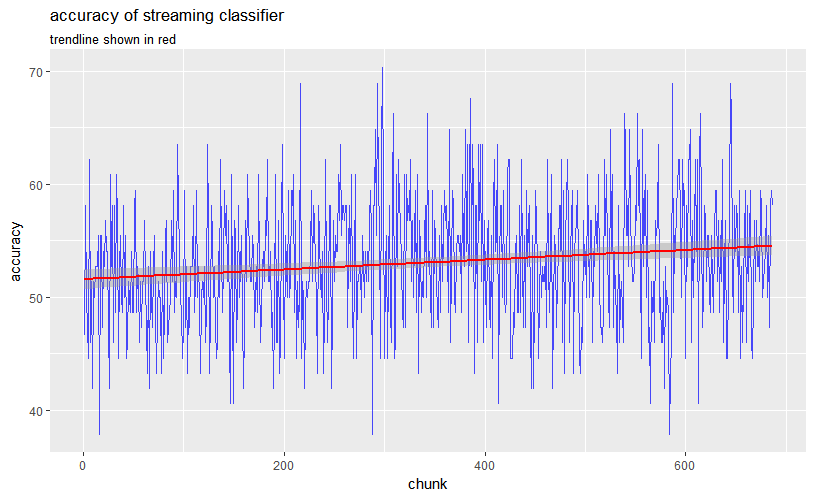
\includegraphics{stream_result}
\caption {Progressive accuracy of the stream classifier}
\label{fig2}
\end {center}
\end {figure}

\pagebreak

\section {Text Classification}

This section involves analysing a collection of tweets collected during the EU referendum. They are labelled 'leave' or 'remain'.



\subsection{Preprocessing}

First, the dataset is loaded into the workspace, along with all the required libraries:

\begin{Schunk}
\begin{Sinput}
> library(dplyr)
> library(tm)
> library(SnowballC)
> library(RColorBrewer)
> library(wordcloud)
> library(ggplot2)
> library(gridExtra)
> library(graph)
> library(Rgraphviz)
> library(RTextTools)
> df <- read.csv("leaveRemainTweets_CW.csv")
\end{Sinput}
\end{Schunk}
The 'leave' and 'remain' tweets are seperated and stored in different objects. We also check that we have captured all tweets by seperating by label (ie there a no unlabelled tweets, or any with labels outwith 'leave' or 'remain'):
\begin{Schunk}
\begin{Sinput}
> #seperate dataframes for leave and remain tweets
> leave_tweets <- df%>%
+   filter(label=="Leave")
> remain_tweets <- df%>%
+   filter(label=="Remain")
> #check we have captured all the tweets
> nrow(df)==(nrow(leave_tweets) + nrow(remain_tweets))
\end{Sinput}
\begin{Soutput}
[1] TRUE
\end{Soutput}
\end{Schunk}
It is important to ensure the dataset is balanced, ie there are a similar number of leave and remain tweets. There are more leave tweets than remain ones, but the difference isn't too great:
\begin{Schunk}
\begin{Sinput}
> nrow(leave_tweets)
\end{Sinput}
\begin{Soutput}
[1] 1254
\end{Soutput}
\begin{Sinput}
> nrow(remain_tweets)
\end{Sinput}
\begin{Soutput}
[1] 1029
\end{Soutput}
\end{Schunk}

In order to analyse the text, a corpus will be built. This will be achieved through a dedicated function defined below. This function performs the following pre-processing steps:

\begin{itemize}
  \item convert the encoding to UTF-8
  \item convert all text to lowercase - the case doesn't give us any extra information.
  \item remove punctuation, numbers and URLs
  \item remove the following common words, none of which convey any real informatiom: "RT","rt","EU","eu","brexit","euref"
  \item remove words CONTAINING the following terms (these are often used in conjunction with a hashtag): 'vote', 'leave', 'remain', 'stronger'.'referendum'.
  \item remove all standard English stopwords
  \item strip out any whitespace.
\end{itemize}

\begin{Schunk}
\begin{Sinput}
> buildCorpus <- function(someText){
+   
+   # build a corpus, and specify the source to be character vectors
+   myCorpus <- Corpus(VectorSource(someText))
+ 
+   myCorpus <- tm_map(myCorpus,
+                      content_transformer(function(x) iconv(x, to='UTF-8',sub='byte')))
+   myCorpus <- tm_map(myCorpus, content_transformer(tolower))
+   # remove punctuation
+   myCorpus <- tm_map(myCorpus, removePunctuation)
+   # remove numbers
+   myCorpus <- tm_map(myCorpus, removeNumbers)
+   # remove URLs
+   removeURL <- function(x) {
+     gsub("http[[:alnum:]]*", "", x)
+   }
+   myCorpus <- tm_map(myCorpus, removeURL)
+   myCorpus <- tm_map(myCorpus, content_transformer(removeURL)) #??
+   # add stopwords
+   myStopwords <- c(stopwords("english"), "RT","rt","EU","eu","brexit","euref")
+   #remove words CONTAINING certain terms
+   myCorpus <- tm_map(myCorpus, content_transformer(gsub), pattern = "*vote*|*leave*|*remain*|*stronger*|*referendum*", replacement = "")
+   # remove stopwords from corpus
+   myCorpus <- tm_map(myCorpus, removeWords, myStopwords)
+   #
+   myCorpus <- tm_map(myCorpus, stripWhitespace)
+   # Return the text corpus
+   return(myCorpus)
+ }
\end{Sinput}
\end{Schunk}
In order to explore the tweets, we will construct a document-term matrix. This will be achieved with the following function. The function returns several useful objects:
\begin{itemize}
  \item the document-term matrix
  \item the term-document matrix
  \item a frequency table for individual words (used to make wordclouds)
  \item the text corpus, as produced by the 'buildCorpus' function
\end{itemize}

\begin{Schunk}
\begin{Sinput}
> #function to build term document matrix, along with other useful objects for analysis
> make_tdm <- function(text_column,minfreq=1){
+   text_column <- iconv(text_column, 'UTF-8', 'ASCII')
+   corpus <- buildCorpus(text_column)
+   # keep for later
+   corpus_copy <- corpus
+   # stem words
+   corpus <- tm_map(corpus, stemDocument)
+   tdm <- TermDocumentMatrix(corpus,control=list(bounds = list(global = c(minfreq,Inf)))) 
+   dtm <- DocumentTermMatrix(corpus,control=list(bounds = list(global = c(minfreq,Inf)))) 
+   m <- as.matrix(tdm)
+   v <- sort(rowSums(m), decreasing = TRUE)
+   d <- data.frame(word = names(v), freq = v)
+   return(list(corpus=corpus,freq_table=d,tdm=tdm , dtm=dtm))
+ }
\end{Sinput}
\end{Schunk}
As the 'maketdm' function outputs a word frequency table, we can use it to produce word clouds for the leave and remain tweets. To avoid repeating tasks, the process for making and plotting wordclouds is defined in dedicated functions.

\begin{Schunk}
\begin{Sinput}
> #make corpuses and tdms from the tweets
> all_tweets <- make_tdm(df$text)
> remain <- make_tdm(remain_tweets$text)
> leave <- make_tdm(leave_tweets$text)
> #function to make wordclouds
> make_wordcloud <- function(freq_tab){
+ wordcloud(words = freq_tab$word, freq = freq_tab$freq, min.freq = 5,max.words=2000,
+ random.order=FALSE, rot.per=0.2,colors=brewer.pal(8, "Dark2"))
+ }
\end{Sinput}
\end{Schunk}
\begin{figure}[H]
\begin{center}

\begin{Schunk}
\begin{Sinput}
> #make wordclouds from the frequency tables
> make_wordcloud(remain$freq_tab)
\end{Sinput}
\end{Schunk}
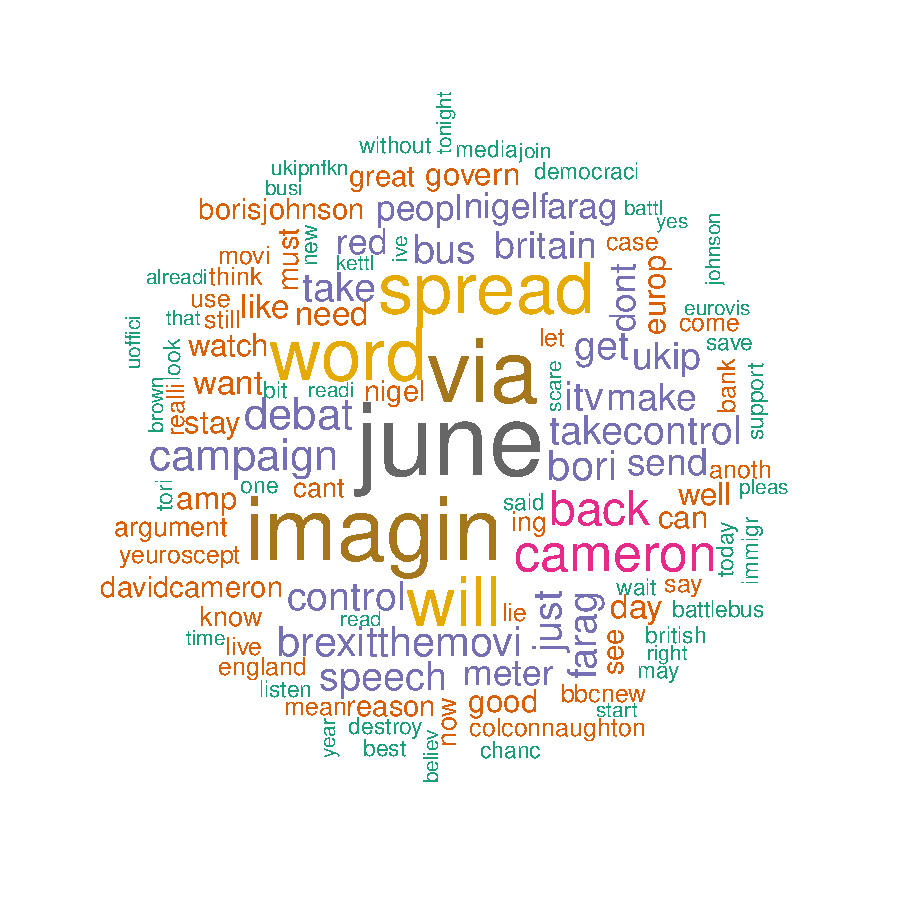
\includegraphics{submission-029}

\caption {Wordclouds for the remain tweets}
\label{fig10}
\end {center}
\end {figure}

\begin{figure}[H]
\begin{center}
\begin{Schunk}
\begin{Sinput}
> make_wordcloud(leave$freq_tab)
\end{Sinput}
\end{Schunk}
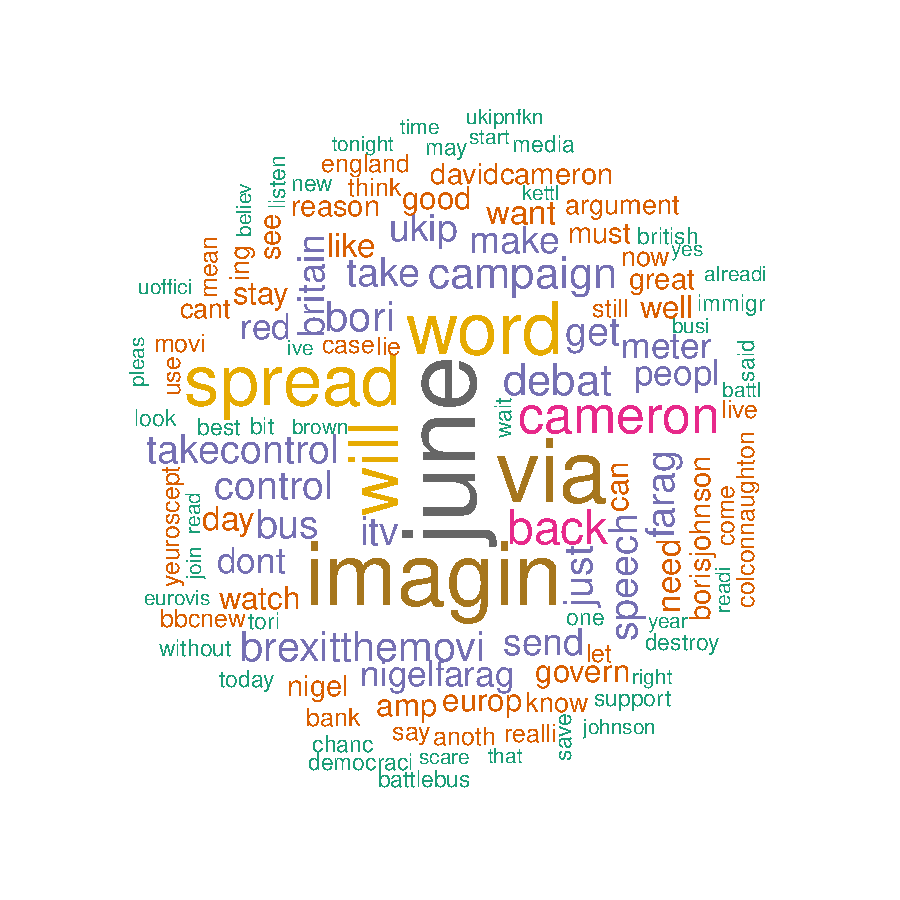
\includegraphics{submission-030}
\caption {Wordclouds for the leave tweets}
\label{fig11}
\end {center}
\end {figure}


In addition to wordclouds, we can plot the most common words for each class of tweet. This is achieve with the function below:
\begin{Schunk}
\begin{Sinput}
> #function to plot wordcounts
> plot_wordcount <- function(freq_tab,title_text){
+   ggplot(head(freq_tab,20), aes(x=word,y=freq))+
+     geom_bar(stat="identity")+
+     labs(title=title_text)+
+     theme(axis.text.x = element_text(angle = 30, hjust = 1))
+ }
> a<-plot_wordcount(all_tweets$freq_table,"most common words for all tweets")
> b<-plot_wordcount(remain$freq_table,"most common words for remain tweets")
> c<-plot_wordcount(leave$freq_table,"most common words for leave tweets")
\end{Sinput}
\end{Schunk}
Referring to figure \ref{fig10}, the most common word for leave tweeters was 'June', suggesting many of them were focused on reinforcing the timing of the referendum - ensuring people remembered to go out and vote. 'via', 'spread' and 'word' were also common, suggesting attempts to get readers to spread the message. The general theme of many of the common words for leave tweets is of trying to increase virality and therefore increase re-tweets.\\
The most common word for remain tweeters was 'say', followed by 'stay', 'will' and 'bori[s]'. These give less of an impression of a common theme compared to the leave tweets. It is not surprising that 'Boris' is mentioned a lot by the remain tweeters since he proved to be a particularly divisive figure during the campaigning. However, the lack of common theme for leave tweets may point to an overall less coordinated campaign and may have been a contributary factor to the final result of the referendum (this is just conjecture however - it must be stressed that the dataset forms a small minority of all tweets from the campaign period).\\
As a humorous aside 'brexitthemovi[e]' was in the top 20 most common words. I don't remember this term from the campaign period but it is interesting to see such a specific term become so popular.

\begin{figure}[H]
\begin{center}
\begin{Schunk}
\begin{Sinput}
> grid.arrange(a,b,c, nrow = 3)
\end{Sinput}
\end{Schunk}
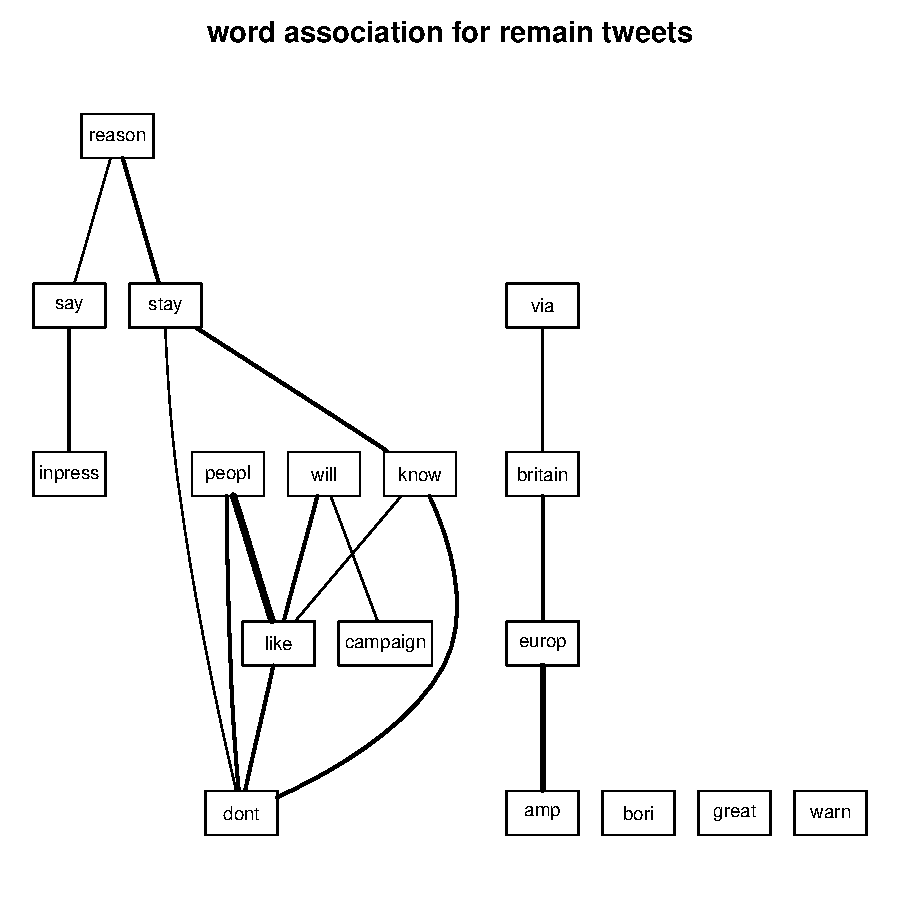
\includegraphics{submission-032}
\caption {Wordcounts for the tweets}
\label{fig10}
\end {center}
\end {figure}

Plotting word associations gives an impression of word usage and gives more insight into common themes between tweets for each class. This is achieved using the build in plotting function for the term-document matrix.\\
For remain tweets (Figure \ref{fig12}), non of the associations are particularly strong when compared to the leave tweets. Of the associations that are present, many seem to convey a negative message such as 'people don't like', or 'don't know'. There doesn't seem to be much evidence of a branded campaign or attempts to spread the message to a wider population.

\begin{figure}[H]
\begin{center}
\begin{Schunk}
\begin{Sinput}
> plot(remain$tdm, term = findFreqTerms(remain$tdm, lowfreq = 10), corThreshold = 0.1,
+      weighting = T, main="word association for remain tweets")
\end{Sinput}
\end{Schunk}
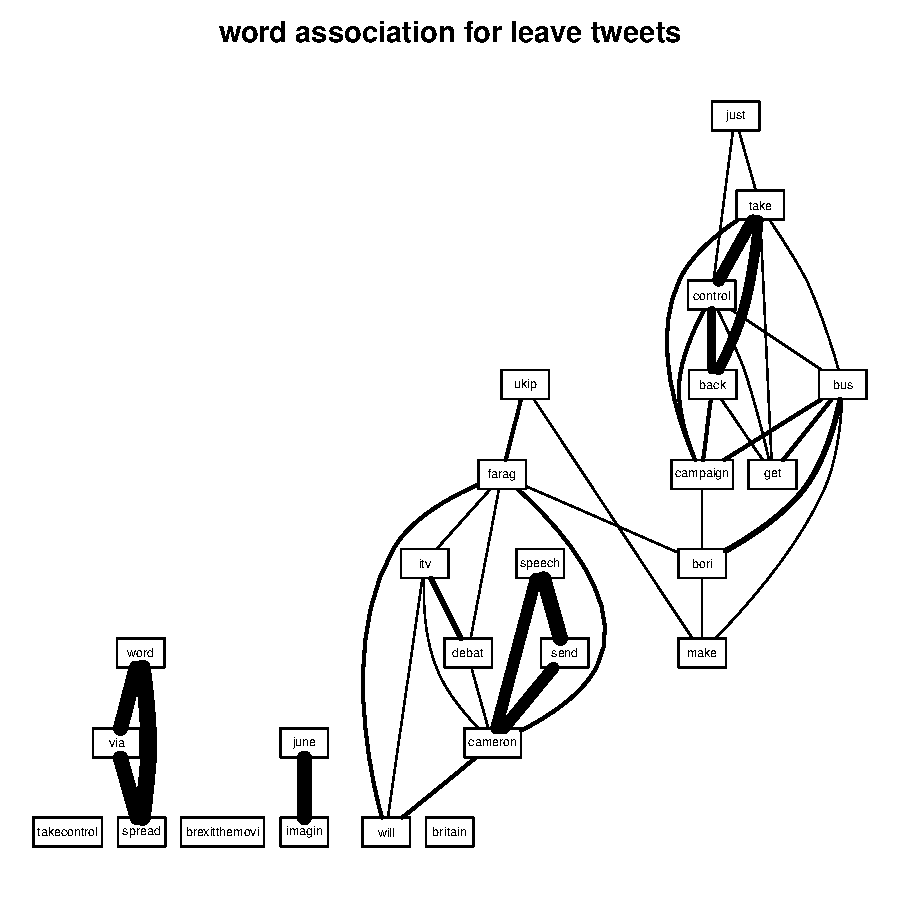
\includegraphics{submission-033}
\caption {Word association for remain tweets}
\label{fig12}
\end {center}
\end {figure}

The leave tweets on the other hand (Figure \ref{fig13}) show some strongly associated words. As suspected previously 'spread', 'word' and 'via' are strongly associated. This suggests a coordinated effort to increase virality of these tweets and make them more visible. 
'Take back control' is another strong grouping. This is a strong and positivley phrased phrase  which would be likely to grab and hold readers' attention (whether we agree with it or not). This contrasts with the negative phrases from the remain tweets which, rather than focusing on why readers should vote remain, seemed more to focus on why readers should \emph{not} vote leave.
Finally 'Cameron', 'Send' and 'Speech' were strongly associated. The reason for this is a little more difficult to ascertain but may relate to one of Cameron's campaign speeches or debates which generally proved to be divisive at the time.
\begin{figure}[H]
\begin{center}
\begin{Schunk}
\begin{Sinput}
> plot(leave$tdm, term = findFreqTerms(leave$tdm, lowfreq = 15), corThreshold = 0.1,
+      weighting = T, main="word association for leave tweets")
\end{Sinput}
\end{Schunk}
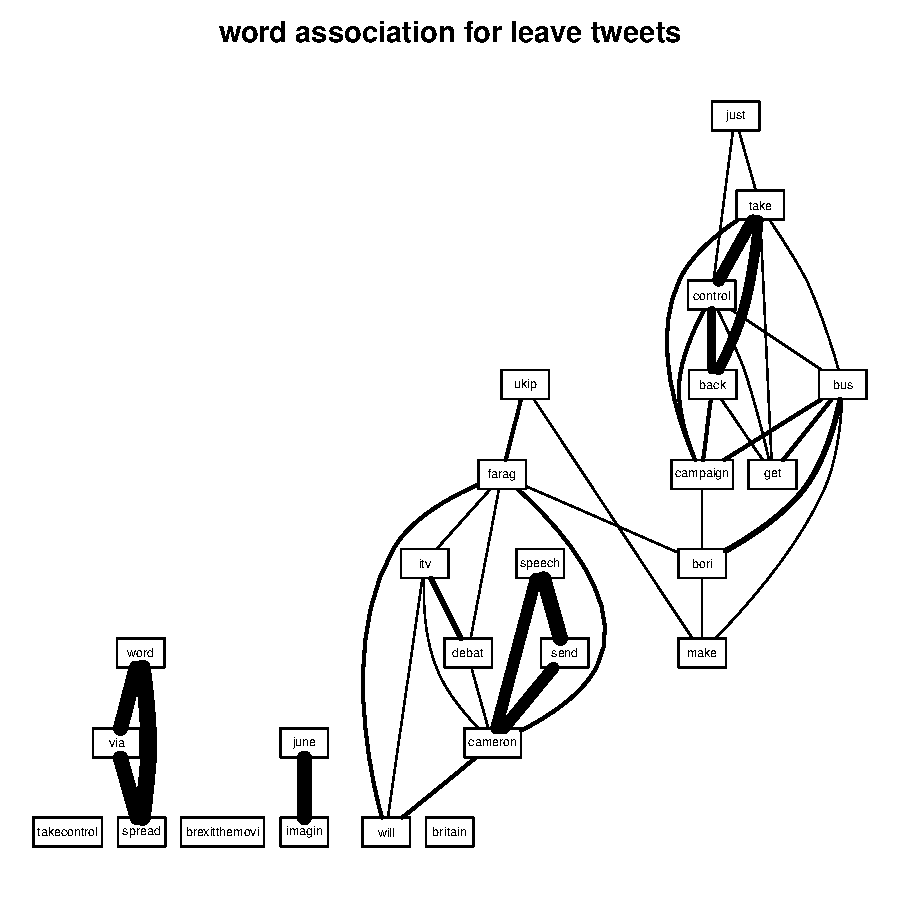
\includegraphics{submission-034}
\caption {Word association for leave tweets}
\label{fig13}
\end {center}
\end {figure}


\subsection{Text Classification}
Most of the preprocessing for text classification is performed within the functions defined earlier. First we create a document-term matrix from all the tweets. We only consider words with a minimum frequency of 10. This removes a significant amount of data, since only 87 unique words are considered.

\begin{Schunk}
\begin{Sinput}
> #transpose the dtm to get word count for each tweet
> dtm<-make_tdm(df$text,10)
> dtm<-dtm$dtm
> #checknumber of columns used for model
> ncol(as.matrix(dtm))
\end{Sinput}
\begin{Soutput}
[1] 87
\end{Soutput}
\end{Schunk}
Using the RTextTools package, the tweets are saved in a container-type object. This automatically performs a train-test split. In this case the training set forms 70\% of the data:
\begin{Schunk}
\begin{Sinput}
> container <- create_container(dtm, df$label,trainSize=1:round(0.7*nrow(df)),
+	 testSize=(round(0.7*nrow(df))+1):nrow(df),virgin=TRUE)
> 
\end{Sinput}
\end{Schunk}
A number of classification models are trained on the data, and evaluated on the test set. RTextTools automatically creates results objects which we can use to evaluate model performance:
\begin{Schunk}
\begin{Sinput}
> #train some models and analyse the results
>set.seed(57)
> models <- train_models(container,algorithms=c("SVM","BAGGING","BOOSTING","RF"))
> results <- classify_models(container, models) #can use for conf matrix

\end{Sinput}
\end{Schunk}
Looking at confusion matrices for each of the model types we get the following:

\begin{figure}[H]
\begin{center}
\begin{Schunk}
\begin{Sinput}
> print("SVM")
\end{Sinput}
\begin{Soutput}
[1] "SVM"
\end{Soutput}
\begin{Sinput}
> table(predicted=results$SVM_LABEL,actual=container@testing_codes)
\end{Sinput}
\begin{Soutput}
         actual
predicted Leave Remain
   Leave    379    270
   Remain    15     21
\end{Soutput}
\begin{Sinput}
> print("Bagging")
\end{Sinput}
\begin{Soutput}
[1] "Bagging"
\end{Soutput}
\begin{Sinput}
> table(predicted=results$BAGGING_LABEL,actual=container@testing_codes)
\end{Sinput}
\begin{Soutput}
         actual
predicted Leave Remain
   Leave    100     41
   Remain   294    250
\end{Soutput}
\begin{Sinput}
> print("Boosting")
\end{Sinput}
\begin{Soutput}
[1] "Boosting"
\end{Soutput}
\begin{Sinput}
> table(predicted=results$LOGITBOOST_LABEL,actual=container@testing_codes)
\end{Sinput}
\begin{Soutput}
         actual
predicted Leave Remain
   Leave    383    272
   Remain    11     19
\end{Soutput}
\begin{Sinput}
> print("Random Forest")
\end{Sinput}
\begin{Soutput}
[1] "Random Forest"
\end{Soutput}
\begin{Sinput}
> table(predicted=results$FORESTS_LABEL,actual=container@testing_codes)
\end{Sinput}
\begin{Soutput}
         actual
predicted Leave Remain
   Leave    105     44
   Remain   289    247
\end{Soutput}
\end{Schunk}

\caption {Confusion matrices for various text classification methods}
\label{fig15}
\end {center}
\end {figure}

None of the cassification results are particularly impressive (Figure \ref{fig15} shows confusion matrices for the four model types tried). Let's take the model with the highest accuracy (the SVM with an accuracy of \textbf{58.4\%} ) and tune the hyperparameters. It should also be noted that the sensitivity for this model type is low since it tends to predict most tweets as type 'Leave'.

 The minimum term frequency is also reduced to incorporate more features into the model training.:
\begin{Schunk}
\begin{Sinput}
>#make minimum term frequency 2
> dtm<-make_tdm(df$text,2)
> dtm<-dtm$dtm
>set.seed(57)
> container <- create_container(dtm, df$label,trainSize=1:round(0.7*nrow(df)), 
+		testSize=(round(0.7*nrow(df))+1):nrow(df),virgin=TRUE)
> library(e1071)
> tuned_svm <- tune.svm(x=container@training_matrix, y=container@training_codes, 
+                       validation.x = container@classification_matrix,
+		 validation.y=container@testing_codes,
+                       gamma=10^(-6:0) , cost=10^(-1:3))
> print('model accuracy = ' )
\end{Sinput}
\begin{Soutput}
[1] "model accuracy = "
\end{Soutput}
\begin{Sinput}
> 1-tuned_svm$best.performance
\end{Sinput}
\begin{Soutput}
[1] 0.5700943
\end{Soutput}
\end{Schunk}

With a final accuracy of \textbf{57.\%}, the tuned model performed \textit{worse} than the initial training run. This is somewhat unexpected and a little puzzling. Several permutations of model type and minimum term frequency were tried and none achieved an accuracy improvement over the original model.\\


\subsection{Conclusions}
The reason for the poor model accuracy may simply be the size of the dataset. With only ~1000 instances for each class, the dataset was relativley small. For text-based data, more instances would normally be used to fit a reliable model. The streaming methods explored in section 2 could be used to train up future models, by pulling data from the Twitter API (or by using a web-scraping tool), allowing for a much larger dataset without memory or storage limitations. It is also likely that altering the preprocessing steps may have given better accuracy. This study was somewhat conservative in removing common words so certain words used frequently in both classes may have added noise to the data, making the classes indistinguishable.


% Clear the page and starte a new page for references 

\clearpage
% The title for the reference section is called References 

\pagebreak

\section{References}\label{pubs}

\printbibliography[heading =none]


\clearpage


\end{document}
